\documentclass[]{informeutn}

% Paquetes adicionales
\usepackage[backend=bibtex, style=alphabetic, sorting=ynt]{biblatex}
\usepackage{csquotes}
\usepackage{listings}
\addbibresource{fuentes.bib}

% Unidades adicionales
\newcommand{\MHz}{\,\mathrm{MHz}}
\newcommand{\kB}{\,\mathrm{kB}}

% Estilos para listados de código
\usepackage{courier}
\usepackage{color}

\definecolor{mygreen}{rgb}{0,0.6,0}
\definecolor{mygray}{rgb}{0.5,0.5,0.5}
\definecolor{mymauve}{rgb}{0.58,0,0.82}
\lstset{ %
  backgroundcolor=\color{white},   % choose the background color; you must add \usepackage{color} or \usepackage{xcolor}
  basicstyle=\scriptsize\ttfamily,        % the size of the fonts that are used for the code
  breakatwhitespace=false,         % sets if automatic breaks should only happen at whitespace
  breaklines=true,                 % sets automatic line breaking
  captionpos=b,                    % sets the caption-position to bottom
  commentstyle=\color{mygreen},    % comment style
  deletekeywords={...},            % if you want to delete keywords from the given language
  escapeinside={\%*}{*)},          % if you want to add LaTeX within your code
  extendedchars=true,              % lets you use non-ASCII characters; for 8-bits encodings only, does not work with UTF-8
  frame=single,                    % adds a frame around the code
  keepspaces=true,                 % keeps spaces in text, useful for keeping indentation of code (possibly needs columns=flexible)
  keywordstyle=\color{blue},       % keyword style
  otherkeywords={*,...},            % if you want to add more keywords to the set
  numbers=left,                    % where to put the line-numbers; possible values are (none, left, right)
  numbersep=5pt,                   % how far the line-numbers are from the code
  numberstyle=\tiny\color{mygray}, % the style that is used for the line-numbers
  rulecolor=\color{black},         % if not set, the frame-color may be changed on line-breaks within not-black text (e.g. comments (green here))
  showspaces=false,                % show spaces everywhere adding particular underscores; it overrides 'showstringspaces'
  showstringspaces=false,          % underline spaces within strings only
  showtabs=false,                  % show tabs within strings adding particular underscores
  stepnumber=1,                    % the step between two line-numbers. If it's 1, each line will be numbered
  stringstyle=\color{mymauve},     % string literal style
  tabsize=2,                       % sets default tabsize to 2 spaces
  title=\lstname                   % show the filename of files included with \lstinputlisting; also try caption instead of title
}

% Metadatos
\materia{Técnicas Digitales II}
\titulo{Trabajo Práctico Nro 1}
\subtitulo{Programación de la placa BluePill usando GNU ARM Toolchain}
\comision{4R1}
\autores{Gastón Grasso 401892\\ Franco Palombo 401910\\ Angelo Prieto 401012}
\fecha{\today}

\begin{document}
  \maketitle
  \tableofcontents
  \setcounter{page}{1}
  \thispagestyle{plain}
  
  \chapter{Introducción}

En este trabajo práctico se aborda la programación de microcontroladores con núcleo ARM 
Cortex-M3, específicamente el \textbf{STM32F103C8T6} presente en la placa \textbf{BluePill}, 
utilizando un enfoque de nivel bajo o \textbf{bare-metal}. El objetivo es comprender el 
funcionamiento del hardware y las herramientas de desarrollo sin capas de abstracción 
intermedias que oculten los detalles de implementación.

\section{Hardware Utilizado}

Para el desarrollo de las actividades se emplearon los siguientes elementos:

\begin{itemize}
    \item \textbf{Placa BluePill}: Basada en el microcontrolador STM32F103C8T6. Cuenta con 
    una frecuencia de reloj de $72 \MHz$, $64 \kB$ de memoria Flash y $20 \kB$ de RAM.
    \item \textbf{Programador ST-Link V2}: Interfaz que permite la grabación y depuración 
    del microcontrolador a través del protocolo SWD.
\end{itemize}

\section{Software y Herramientas}

Se utilizó el ecosistema de herramientas estándar de GNU para sistemas embebidos:

\begin{itemize}
    \item \textbf{GNU ARM Toolchain}: Colección de compiladores, enlazadores y utilidades 
    para la arquitectura ARM (\texttt{arm-none-eabi-gcc}).
    \item \textbf{Make}: Herramienta para la automatización del proceso de compilación.
    \item \textbf{OpenOCD}: Software para la comunicación con el programador y el 
    microcontrolador.
    \item \textbf{GDB}: Depurador estándar para inspeccionar el estado del programa en 
    tiempo de ejecución.
\end{itemize}

  \chapter{Desarrollo}
\label{chap:desarrollo}

El proyecto principal consistió en implementar un \textbf{Blink LED} utilizando el LED 
integrado en la placa BluePill, el cual se encuentra conectado al pin \textbf{PC13}.

\section{Configuración de Periféricos}

Para controlar el LED, es necesario configurar el puerto C y el pin 13. El proceso 
implica los siguientes pasos:

\begin{enumerate}
    \item \textbf{Habilitación del reloj (Clock Gating)}: Se debe habilitar el reloj para 
    el puerto C en el registro \texttt{RCC\_APB2ENR}.
    \item \textbf{Configuración del pin}: Se configura el pin PC13 como salida en el 
    registro \texttt{GPIOC\_CRH}.
\end{enumerate}

\section{Archivos del Proyecto}

El firmware se compone de tres archivos fundamentales:

\begin{itemize}
    \item \texttt{main.c}: Contiene la lógica principal del programa y el bucle de parpadeo.
    \item \texttt{crt.s}: Archivo de \textit{startup} en ensamblador que inicializa el 
    puntero de pila y el vector de interrupciones.
    \item \texttt{linker.ld}: Script del enlazador que define la distribución de la 
    memoria Flash y RAM.
\end{itemize}

\section{Proceso de Compilación y Grabación}

Se utilizó un \texttt{Makefile} para automatizar la generación del binario. El flujo 
consiste en compilar los archivos fuente a objetos, enlazarlos para generar un archivo 
ELF, y finalmente extraer el binario (\texttt{.bin}).

Para la grabación se utilizó OpenOCD con el comando:
\begin{verbatim}
openocd -f interface/stlink.cfg -f target/stm32f1x.cfg
\end{verbatim}
seguido de los comandos de grabación en la consola de OpenOCD.

  \chapter{Conclusiones}

El desarrollo de este trabajo práctico permitió familiarizarse con el flujo de trabajo 
estándar para la programación de sistemas embebidos ARM sin depender de entornos 
integrados propietarios. Se logró comprender la importancia de los archivos de 
\textit{startup} y el script del enlazador para el inicio correcto del microcontrolador.

El uso de herramientas como Make y OpenOCD facilita la integración en sistemas de 
desarrollo flexibles y potentes, permitiendo un control total sobre el proceso de 
generación de código y depuración. La configuración directa de registros para el control 
de GPIO sentó las bases para el manejo de periféricos más complejos en futuros trabajos.

  \chapter{Anexos}

\section{Código Fuente}

En esta sección se adjunta el código fuente completo del proyecto Blink LED.

\subsection{Archivo main.c}
\lstinputlisting[language=C, caption={Lógica principal en C}]{sources/blink_led/src/main.c}

\subsection{Archivo crt.s}
\lstinputlisting[language=C, caption={Archivo de startup en ensamblador}]{sources/blink_led/src/crt.s}

\subsection{Script del Enlazador (linker.ld)}
\lstinputlisting[language=C, caption={Configuración del enlazador}]{sources/blink_led/src/linker.ld}

\subsection{Makefile}
\lstinputlisting[language=make, caption={Automatización de la compilación}]{sources/blink_led/Makefile}

\newpage

\section{Extractos de documentos}

\subsection{Mapa de memoria}
\label{annex:mapa_memoria}

\begin{figure}[!ht]
    \centering
        \includegraphics[page=34, trim=4cm 4.8cm 2cm 5.45cm, clip=true, height=17cm]{../commons/stm32f103c8.pdf}
    \caption{mapa de memoria del STM32F103x8.}
\end{figure}


  
  \nocite{*}
  \printbibliography[heading=bibnumbered, title={Fuentes}]
  
\end{document}
